\documentclass{article}
\usepackage{graphicx}
\usepackage{amsmath}
\usepackage{booktabs}
\usepackage{siunitx}
\usepackage{float}

\title{Homework 1 - ET4369 Nyquist Rate Data Converters}
\author{Daniel Tyukov \\ Student Number: 5714699 \\ Electrical Engineering, TU Delft}
\date{February 2026}

\begin{document}

\maketitle

\tableofcontents

  \section{Anti-Alias Filtering}

  \textbf{Given:} Anti-alias filter $H(s)$ with $0$\,dB passband, $-80$\,dB/decade roll-off beyond cutoff at $f_B = 1$\,MHz,
  followed by an ideal sampler at rate $f_s$.

  \subsection{Part (a): Minimum $f_s$ for $>70$\,dB alias rejection}

  After sampling at $f_s$, a signal component at frequency $f_a$ aliases into the baseband. The worst-case in-band alias
  originates from frequency
  \begin{equation}
      f_a = f_s - f_B
  \end{equation}
  which folds back to $f_B$ (the edge of the signal band). Since this is the aliasing frequency closest to the passband, it
  experiences the least filter attenuation and therefore sets the requirement.

  The filter attenuation at any frequency $f > f_B$ is
  \begin{equation}
      \bigl|H(f)\bigr|_{\mathrm{dB}} = -80 \cdot \log_{10}\!\left(\frac{f}{f_B}\right)
  \end{equation}

  Requiring $>70$\,dB of attenuation at $f_a = f_s - f_B$:
  \begin{align}
      80 \cdot \log_{10}\!\left(\frac{f_s - f_B}{f_B}\right) &> 70 \\[6pt]
      \log_{10}\!\left(\frac{f_s - f_B}{f_B}\right) &> \frac{7}{8} \\[6pt]
      \frac{f_s - f_B}{f_B} &> 10^{7/8} \\[6pt]
      f_s &> f_B\bigl(1 + 10^{7/8}\bigr)
  \end{align}

  Evaluating numerically ($10^{7/8} \approx 7.499$):
  \begin{equation}
      \boxed{f_{s,\min} = \bigl(1 + 10^{7/8}\bigr) \times 1\,\text{MHz} \approx 8.50\,\text{MHz}}
  \end{equation}

  The resulting oversampling ratio is
  \begin{equation}
      \boxed{\mathrm{OSR} = \frac{f_s / 2}{f_B} = \frac{8.50}{2 \times 1} \approx 4.25}
  \end{equation}

  \subsection{Part (b): Required OSR with $-60$\,dB/decade roll-off}

  With a reduced roll-off of $-60$\,dB/decade, the same analysis gives:
  \begin{align}
      60 \cdot \log_{10}\!\left(\frac{f_s - f_B}{f_B}\right) &> 70 \\[6pt]
      \log_{10}\!\left(\frac{f_s - f_B}{f_B}\right) &> \frac{7}{6} \\[6pt]
      \frac{f_s - f_B}{f_B} &> 10^{7/6} \\[6pt]
      f_s &> f_B\bigl(1 + 10^{7/6}\bigr)
  \end{align}

  Evaluating numerically ($10^{7/6} = 10 \cdot 10^{1/6} \approx 14.68$):
  \begin{equation}
      f_{s,\min} = \bigl(1 + 14.68\bigr) \times 1\,\text{MHz} \approx 15.68\,\text{MHz}
  \end{equation}
  \begin{equation}
      \boxed{\mathrm{OSR} = \frac{f_s / 2}{f_B} = \frac{15.68}{2 \times 1} \approx 7.84}
  \end{equation}

  \section{State-of-the-Art Data Converters}

  Three recently published high-performance A/D converter papers from the \textit{IEEE Journal of Solid-State Circuits} (2022)
  are reviewed below.

  %% ============================================================
  %% PAPER 1
  %% ============================================================
  \subsection{Paper 1: OTA-Free 1--1 MASH ADC}

  \subsubsection*{(a) IEEE Reference}
  S.~T.~Chandrasekaran, S.~P.~Bhanushali, S.~Pietri and A.~Sanyal,
  ``OTA-Free 1--1 MASH ADC Using Fully Passive Noise-Shaping SAR \& VCO ADC,''
  \textit{IEEE J. Solid-State Circuits}, vol.~57, no.~4, pp.~1100--1111, Apr.~2022.

  \subsubsection*{(b) Resolution, Sampling Rate, and Power}
  \begin{itemize}
      \item SNDR: 71.5\,dB $\;\Rightarrow\;$ ENOB $\approx 11.6$\,bits; Dynamic range: 75.8\,dB
      \item Sampling rate: 24\,MS/s (signal bandwidth 1.1\,MHz at OSR\,=\,11)
      \item Power consumption: 0.16\,mW from a 1.1\,V supply
  \end{itemize}

  \subsubsection*{(c) Technology and Chip Area}
  \begin{itemize}
      \item Technology: 65\,nm CMOS
      \item Active core area: 0.045\,mm\textsuperscript{2}
  \end{itemize}

  \subsubsection*{(d) Architecture and Application}
  \begin{itemize}
      \item Architecture: 1--1 MASH oversampling ADC with a fully passive noise-shaping SAR as the first stage and a ring VCO as
   the second stage. The design is OTA-free and highly digital/scaling-friendly.
      \item Application: Low-power, medium-bandwidth applications such as sensor interfaces and IoT devices.
  \end{itemize}

  \subsubsection*{(e) Battery Life Estimate}
  \[
      t = \frac{E_{\text{battery}}}{P} = \frac{5\,\text{Wh}}{0.16\,\text{mW}} = 31{,}250\,\text{hours} \approx
  \mathbf{1{,}302\,\text{days}\;\approx\;3.6\,\text{years}}
  \]

  %% ============================================================
  %% PAPER 2
  %% ============================================================
  \subsection{Paper 2: 7-Bit Two-Step Flash ADC}

  \subsubsection*{(a) IEEE Reference}
  D.-R.~Oh, M.-J.~Seo and S.-T.~Ryu,
  ``A 7-Bit Two-Step Flash ADC With Sample-and-Hold Sharing Technique,''
  \textit{IEEE J. Solid-State Circuits}, vol.~57, no.~9, pp.~2791--2801, Sep.~2022.

  \subsubsection*{(b) Resolution, Sampling Rate, and Power}
  \begin{itemize}
      \item Resolution: 7\,bits (ENOB 6.34 at Nyquist input)
      \item Sampling rate: 3\,GS/s (two-channel time-interleaved)
      \item Power consumption: 6.8\,mW from a 0.9\,V supply
  \end{itemize}

  \subsubsection*{(c) Technology and Chip Area}
  \begin{itemize}
      \item Technology: 40\,nm CMOS
      \item Core area: 0.03\,mm\textsuperscript{2} (including offset calibration circuitry)
  \end{itemize}

  \subsubsection*{(d) Architecture and Application}
  \begin{itemize}
      \item Architecture: Two-step flash ADC (2.5-bit coarse + 5-bit fine) with sample-and-hold sharing technique and
  reference-embedding eight-time interpolating fine ADC. Two-channel time-interleaved for 3\,GS/s operation.
      \item Application: High-speed wireline/wireless communication receivers requiring wide effective resolution bandwidth
  (ERBW up to 7\,GHz).
  \end{itemize}

  \subsubsection*{(e) Battery Life Estimate}
  \[
      t = \frac{5\,\text{Wh}}{6.8\,\text{mW}} = 735.3\,\text{hours} \approx \mathbf{30.6\,\text{days}}
  \]

  %% ============================================================
  %% PAPER 3
  %% ============================================================
  \subsection{Paper 3: SAR-Assisted Noise-Shaping Pipeline ADC}

  \subsubsection*{(a) IEEE Reference}
  Y.~Zhang, J.~Zhang, S.~Liu, R.~Ding, Y.~Zhu, C.-H.~Chan and R.~P.~Martins,
  ``A 20 MHz Bandwidth 79 dB SNDR SAR-Assisted Noise-Shaping Pipeline ADC With Gain and Offset Calibrations,''
  \textit{IEEE J. Solid-State Circuits}, vol.~57, no.~3, pp.~745--756, Mar.~2022.

  \subsubsection*{(b) Resolution, Sampling Rate, and Power}
  \begin{itemize}
      \item SNDR: 79.1\,dB $\;\Rightarrow\;$ ENOB $\approx 12.8$\,bits; Bandwidth: 20\,MHz
      \item Sampling rate: 260\,MS/s (OSR\,=\,6.5)
      \item Power consumption: 3.1\,mW from a 1\,V supply
  \end{itemize}

  \subsubsection*{(c) Technology and Chip Area}
  \begin{itemize}
      \item Technology: 28\,nm CMOS
      \item Active area: 0.037\,mm\textsuperscript{2}
  \end{itemize}

  \subsubsection*{(d) Architecture and Application}
  \begin{itemize}
      \item Architecture: Second-order SAR-assisted noise-shaping pipeline ADC with error-feedback (EF) structure, optimized NTF
   zeros, background inter-stage gain and offset calibrations, and partial interleaving.
      \item Application: Wideband communication baseband processing and software-defined radio.
  \end{itemize}

  \subsubsection*{(e) Battery Life Estimate}
  \[
      t = \frac{5\,\text{Wh}}{3.1\,\text{mW}} = 1{,}612.9\,\text{hours} \approx \mathbf{67.2\,\text{days}}
  \]

  %% ============================================================
  %% SUMMARY TABLE
  %% ============================================================
  \subsection{Summary Comparison}

  \begin{table}[H]
  \centering
  \caption{Comparison of the three selected ADCs.}
  \begin{tabular}{@{}lccc@{}}
  \toprule
  \textbf{Parameter} & \textbf{Paper 1} & \textbf{Paper 2} & \textbf{Paper 3} \\
  \midrule
  Architecture    & NS-SAR + VCO MASH  & Two-step flash (TI)  & NS pipeline (SAR-assisted) \\
  Technology      & 65\,nm             & 40\,nm               & 28\,nm \\
  Resolution      & 11.6-bit ENOB      & 7-bit (6.34 ENOB)    & 12.8-bit ENOB \\
  Sampling rate   & 24\,MS/s           & 3\,GS/s              & 260\,MS/s \\
  Bandwidth       & 1.1\,MHz           & 1.5\,GHz (Nyquist)   & 20\,MHz \\
  Power           & 0.16\,mW           & 6.8\,mW              & 3.1\,mW \\
  Area            & 0.045\,mm$^2$      & 0.03\,mm$^2$         & 0.037\,mm$^2$ \\
  Supply          & 1.1\,V             & 0.9\,V               & 1\,V \\
  Battery life    & $\approx$3.6\,yr   & $\approx$30.6\,days  & $\approx$67.2\,days \\
  \bottomrule
  \end{tabular}
  \end{table}


  \section{Quantization Noise Power Calculation for a Ramp Input Signal}

  \subsection{Part (a): Ideal 3-bit Mid-Tread Quantizer}

  \subsubsection{Setup}

  An ideal 3-bit mid-tread quantizer has $2^3 = 8$ output levels at $D_\text{out} \in \{-4, -3, -2, -1, 0, 1, 2, 3\}$ (in units
  of $\Delta$), where $\Delta$ is the quantization step size. The decision boundaries are at $\{-3.5, -2.5, -1.5, -0.5, 0.5,
  1.5, 2.5\}\Delta$, and the full-scale range is $\text{FSR} = 2^B \cdot \Delta = 8\Delta$, spanning the input range
  $[-4.5\Delta,\; 3.5\Delta)$.

  The ramp input is:
  \begin{equation}
      x(t) = -4.5\Delta + 8\Delta \cdot \frac{t}{t_1}, \quad t \in [0,\; t_1]
  \end{equation}

  \subsubsection{Quantization Error}

  Within each quantization step centered at output level $k\Delta$, the input $x$ ranges over an interval of width $\Delta$. The
   quantization error is:
  \begin{equation}
      e(x) = Q(x) - x = k\Delta - x
  \end{equation}
  which is a linear function that decreases from $+\Delta/2$ to $-\Delta/2$ as $x$ traverses the step. Since the ramp input
  sweeps the full scale range uniformly, the error signal is a \textbf{periodic sawtooth wave} with 8 complete periods (one per
  quantization step), each with peak-to-peak amplitude $\Delta$.

  The quantization error as a function of normalized time is shown in Figure~\ref{fig:p3a}.

  \begin{figure}[H]
      \centering
      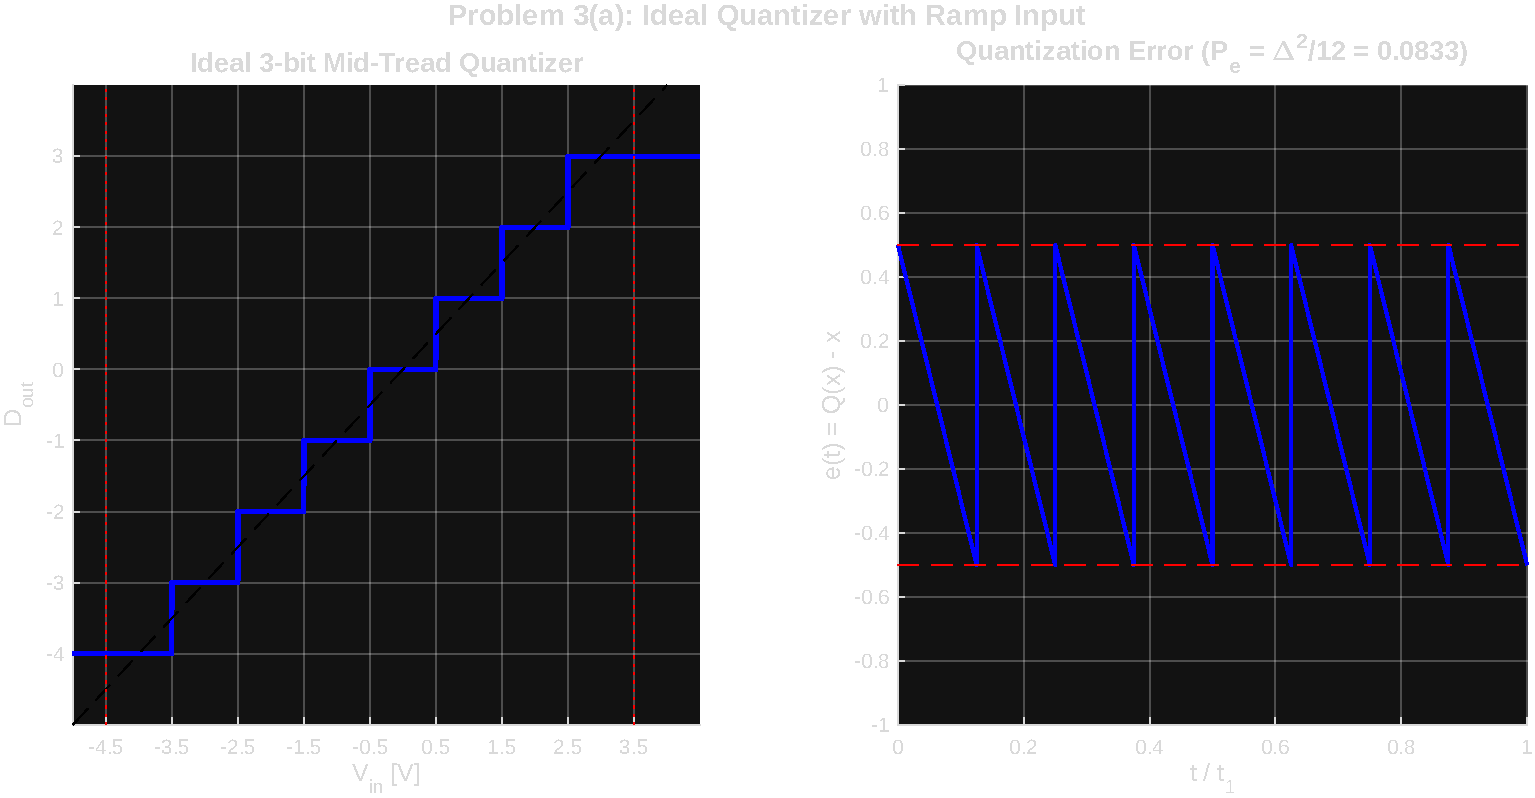
\includegraphics[width=0.95\textwidth]{p3a_ideal_quantizer.pdf}
      \caption{Ideal 3-bit mid-tread quantizer: transfer characteristic (left) and quantization error for ramp input (right).}
      \label{fig:p3a}
  \end{figure}

  \subsubsection{Noise Power Calculation}

  The quantization noise power is the mean-square value of the error over the full ramp:
  \begin{equation}
      P_e = \frac{1}{\text{FSR}} \int_{-4.5\Delta}^{3.5\Delta} e^2(x)\, dx
  \end{equation}

  Since each of the 8 steps contributes an identical integral, we compute the integral for one step. For a step centered at
  $k\Delta$ with input range $[(k-\tfrac{1}{2})\Delta,\; (k+\tfrac{1}{2})\Delta)$:
  \begin{equation}
      \int_{(k-\frac{1}{2})\Delta}^{(k+\frac{1}{2})\Delta} (k\Delta - x)^2\, dx
      = \int_{-\Delta/2}^{\Delta/2} u^2\, du
      = \left[\frac{u^3}{3}\right]_{-\Delta/2}^{\Delta/2}
      = \frac{2}{3}\left(\frac{\Delta}{2}\right)^3
      = \frac{\Delta^3}{12}
  \end{equation}

  Summing over all 8 steps:
  \begin{equation}
      P_e = \frac{1}{8\Delta} \cdot 8 \cdot \frac{\Delta^3}{12} = \boxed{\frac{\Delta^2}{12}}
  \end{equation}

  This is \textbf{exactly} the standard quantization noise model result $\Delta^2/12$, confirmed numerically by MATLAB ($P_e =
  0.0833$).

  \subsubsection{Discussion}

  The ramp input is special: it traverses each quantization bin uniformly, spending equal time in every step. The resulting
  error is a perfect sawtooth wave, equivalent to a uniform distribution on $[-\Delta/2, +\Delta/2]$, which is exactly the
  assumption of the statistical quantization noise model.

  \textbf{Why didn't we use this approach for the sinusoidal case?}
  A sinusoidal input does \emph{not} traverse quantization bins uniformly. Near its peaks ($\pm A$), the sinusoid's slope is
  small, so it spends more time in those bins; near zero crossings, it moves quickly. The input probability density of a
  sinusoid is the arc-sine distribution, not uniform. Therefore, the deterministic sawtooth analysis does not directly apply to
  a sinusoid, and one must instead rely on the statistical approximation (assuming the quantization error is uniformly
  distributed and uncorrelated with the signal), which holds well when the signal spans many quantization levels and the
  frequency is not harmonically related to the sampling frequency.

  \subsection{Part (b): Broken Quantizer (Missing Codes 0 and 1)}

  \subsubsection{Identifying the Defect}

  From the given figure, the ``broken'' quantizer has the following transfer characteristic:

  \begin{table}[H]
  \centering
  \begin{tabular}{ccc}
  \toprule
  Output Code $D_\text{out}$ & Input Range $V_\text{in}$ & Step Width \\
  \midrule
  $-4$ & $[-4.5\Delta,\; -3.5\Delta)$ & $\Delta$ \\
  $-3$ & $[-3.5\Delta,\; -2.5\Delta)$ & $\Delta$ \\
  $-2$ & $[-2.5\Delta,\; -1.5\Delta)$ & $\Delta$ \\
  $-1$ & $[-1.5\Delta,\; +1.5\Delta)$ & $3\Delta$ \\
  $+2$ & $[+1.5\Delta,\; +2.5\Delta)$ & $\Delta$ \\
  $+3$ & $[+2.5\Delta,\; +3.5\Delta)$ & $\Delta$ \\
  \bottomrule
  \end{tabular}
  \caption{Transfer characteristic of the broken quantizer. Codes 0 and 1 are missing.}
  \label{tab:broken_quant}
  \end{table}

  The step at $D_\text{out} = -1$ is \textbf{three times wider} than normal ($3\Delta$ instead of $\Delta$), absorbing the input
   ranges that would normally correspond to codes 0 and 1.

  \subsubsection{Quantization Error}

  The quantization error and its sketch are shown in Figure~\ref{fig:p3b}.

  \begin{figure}[H]
      \centering
      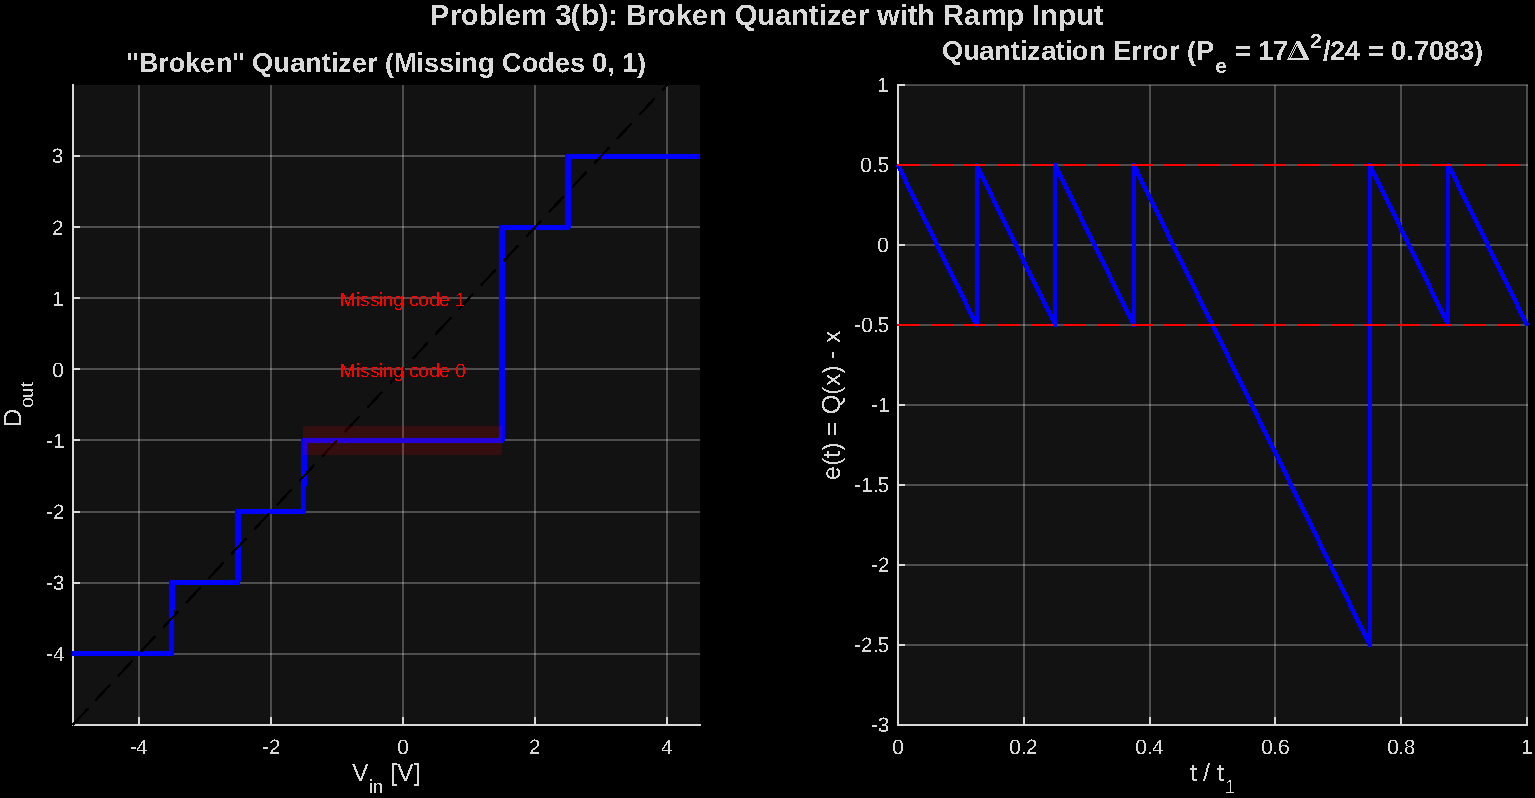
\includegraphics[width=0.95\textwidth]{p3b_broken_quantizer.pdf}
      \caption{Broken quantizer: transfer characteristic (left) and quantization error for ramp input (right). The error greatly
   exceeds $\pm\Delta/2$ during the wide step.}
      \label{fig:p3b}
  \end{figure}

  For the 5 normal-width steps, the error is the standard sawtooth from $+\Delta/2$ to $-\Delta/2$. For the triple-width step at
   $D_\text{out} = -1$:
  \begin{equation}
      e(x) = (-1)\Delta - x, \quad x \in [-1.5\Delta,\; 1.5\Delta)
  \end{equation}
  \begin{itemize}
      \item At $x = -1.5\Delta$: $e = -\Delta - (-1.5\Delta) = +\frac{\Delta}{2}$
      \item At $x = +1.5\Delta$: $e = -\Delta - 1.5\Delta = -\frac{5\Delta}{2}$
  \end{itemize}
  The error grows far beyond the normal $\pm\Delta/2$ bounds, reaching $-5\Delta/2$ at the end of the wide step.

  \subsubsection{Noise Power Calculation}

  The total noise power is:
  \begin{equation}
      P_e = \frac{1}{\text{FSR}} \left[\sum_{\text{5 normal steps}} \int e^2\, dx + \int_{\text{wide step}} e^2\, dx \right]
  \end{equation}

  \textbf{Normal steps} (5 steps of width $\Delta$): each contributes $\Delta^3/12$:
  \begin{equation}
      \sum_{\text{normal}} \int e^2\, dx = 5 \cdot \frac{\Delta^3}{12} = \frac{5\Delta^3}{12}
  \end{equation}

  \textbf{Wide step} (output $= -\Delta$, input $\in [-1.5\Delta,\; 1.5\Delta)$):
  \begin{align}
      \int_{-1.5\Delta}^{1.5\Delta} (-\Delta - x)^2\, dx
      &= \int_{-1.5\Delta}^{1.5\Delta} (\Delta^2 + 2\Delta x + x^2)\, dx \nonumber \\
      &= \left[\Delta^2 x + \Delta x^2 + \frac{x^3}{3}\right]_{-1.5\Delta}^{1.5\Delta} \nonumber \\
      &= \left(1.5\Delta^3 + 2.25\Delta^3 + \frac{3.375\Delta^3}{3}\right) - \left(-1.5\Delta^3 + 2.25\Delta^3 -
  \frac{3.375\Delta^3}{3}\right) \nonumber \\
      &= (1.5 + 2.25 + 1.125)\Delta^3 - (-1.5 + 2.25 - 1.125)\Delta^3 \nonumber \\
      &= 4.875\Delta^3 - (-0.375)\Delta^3 = \frac{21\Delta^3}{4}
  \end{align}

  \textbf{Total noise power:}
  \begin{equation}
      P_e = \frac{1}{8\Delta}\left(\frac{5\Delta^3}{12} + \frac{21\Delta^3}{4}\right)
      = \frac{1}{8\Delta} \cdot \frac{5\Delta^3 + 63\Delta^3}{12}
      = \frac{68\Delta^2}{96}
      = \boxed{\frac{17\Delta^2}{24}}
  \end{equation}

  This result is confirmed numerically by MATLAB ($P_e = 0.7083$).

  \subsubsection{Comparison}

  The broken quantizer has a noise power of $17\Delta^2/24$, compared to $\Delta^2/12$ for the ideal quantizer:
  \begin{equation}
      \frac{P_{e,\text{broken}}}{P_{e,\text{ideal}}} = \frac{17\Delta^2/24}{\Delta^2/12} = \frac{17}{2} = 8.5
  \end{equation}
  

  \section{Quantization Noise Model Validation}

  

  \subsection{Signal Generation}

  Four test signals of 10{,}000 samples are generated, all with equal power $P = A^2/2 = 0.5$:
  \begin{enumerate}
      \item \textbf{Sinusoidal:} $x_1(n) = A\cos(2\pi \cdot 67/2048 \cdot n)$, $A = 1$
      \item \textbf{Uniform:} $x_2 \sim \mathcal{U}[-a,\, a]$, $a = \sqrt{3P} = \sqrt{3/2} \approx 1.225$
      \item \textbf{Gaussian:} $x_3 \sim \mathcal{N}(0,\, \sigma^2)$, $\sigma = \sqrt{P} = 1/\sqrt{2} \approx 0.707$
      \item \textbf{ReLU Gaussian:} $x_4 = \max(\mathcal{N}(0,\, \sigma_{hw}^2),\, 0)$, $\sigma_{hw} = \sqrt{2P} = 1$
  \end{enumerate}

  The power-matching conditions follow from:
  \begin{align}
      \text{Uniform:} \quad E[x^2] &= \frac{a^2}{3} = P \;\Rightarrow\; a = \sqrt{3P} \\
      \text{Gaussian:} \quad E[x^2] &= \sigma^2 = P \;\Rightarrow\; \sigma = \sqrt{P} \\
      \text{ReLU Gaussian:} \quad E[x^2] &= \frac{\sigma_{hw}^2}{2} = P \;\Rightarrow\; \sigma_{hw} = \sqrt{2P}
  \end{align}

  \subsection{SQNR vs Loading Factor (B = 10)}

  Figure~\ref{fig:sqnr_lf_B10} shows the range-precision trade-off for all four signals at $B = 10$ bits. The loading factor is
  defined as $\text{LF} = (V_\text{FSR}/2) / x_\text{rms}$.

  \begin{figure}[H]
      \centering
      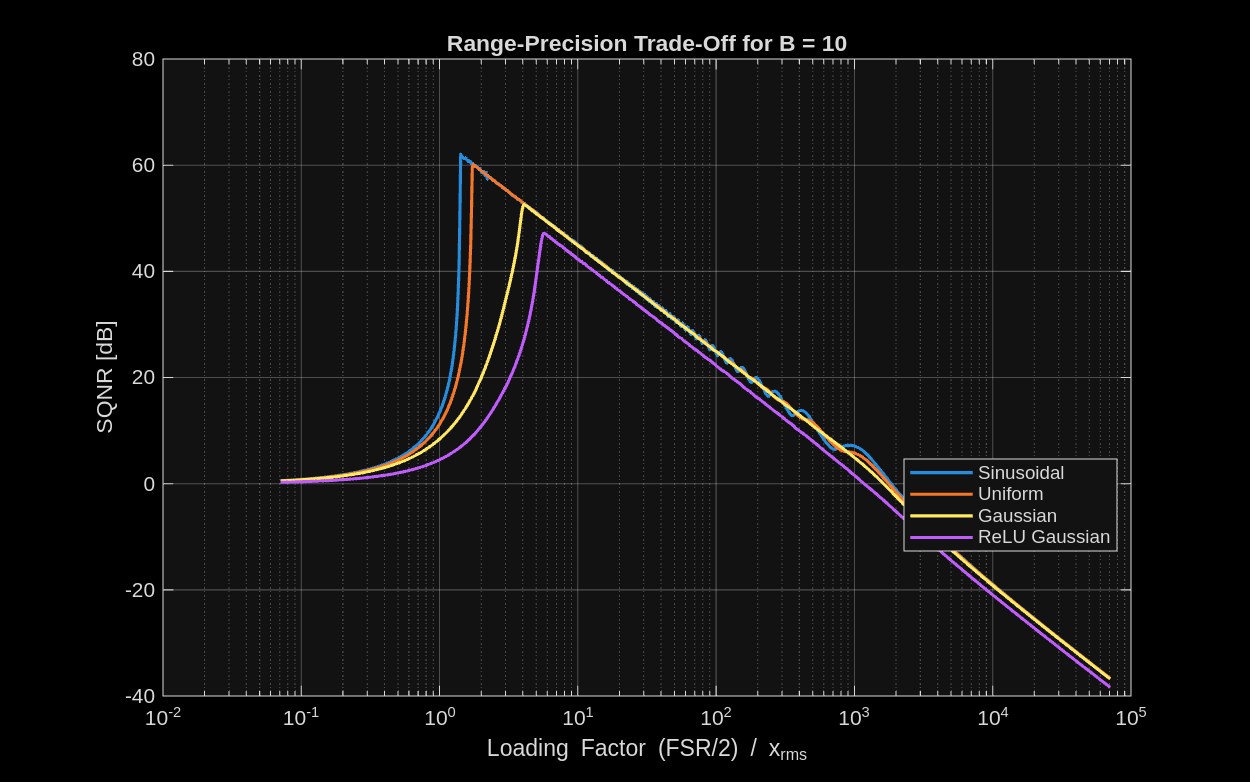
\includegraphics[width=0.85\textwidth]{p4_sqnr_vs_lf_B10.png}
      \caption{SQNR vs loading factor for all four input signals at $B = 10$.}
      \label{fig:sqnr_lf_B10}
  \end{figure}

  At low loading factors the quantizer overloads (clipping), degrading SQNR. At high loading factors the signal occupies only a
  few quantization levels, wasting resolution. The sinusoidal input achieves the highest peak SQNR because its bounded amplitude
   avoids clipping at the optimal loading factor. The Gaussian and ReLU Gaussian signals, having unbounded tails, require a
  larger FSR to avoid clipping and therefore achieve lower peak SQNR.

  \subsection{SQNR vs Loading Factor Across Resolutions (Sinusoidal)}

  Figure~\ref{fig:sqnr_lf_allB} shows how the SQNR curve shifts upward by approximately 6\,dB per additional bit, consistent
  with the theoretical $\text{SQNR} = 6.02B + 1.76$\,dB for a full-scale sinusoid.

  \begin{figure}[H]
      \centering
      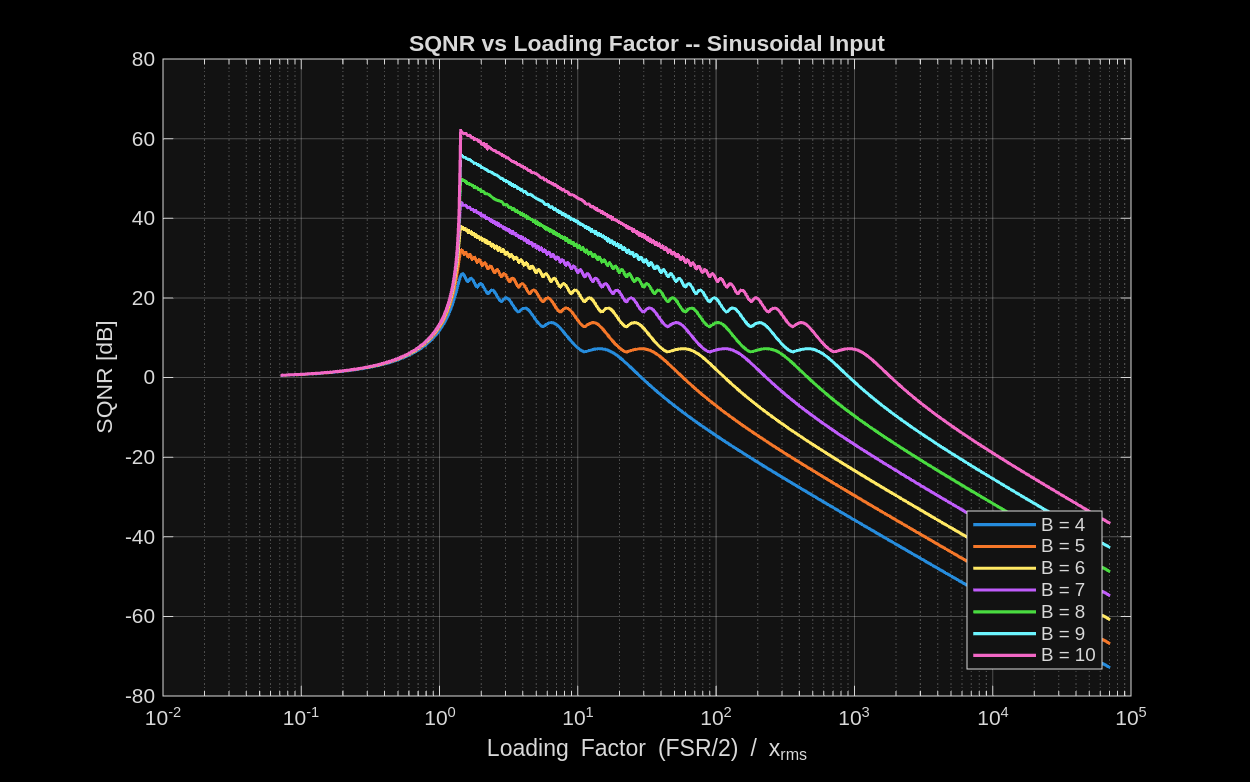
\includegraphics[width=0.85\textwidth]{p4_sqnr_vs_lf_allB_sine.png}
      \caption{SQNR vs loading factor for sinusoidal input at resolutions $B = 4\ldots10$.}
      \label{fig:sqnr_lf_allB}
  \end{figure}

  \subsection{Optimal SQNR and Loading Factor vs Resolution}

  Figure~\ref{fig:optimal} shows the peak SQNR and the corresponding optimal loading factor as a function of bit resolution for
  each signal type.

  \begin{figure}[H]
      \centering
      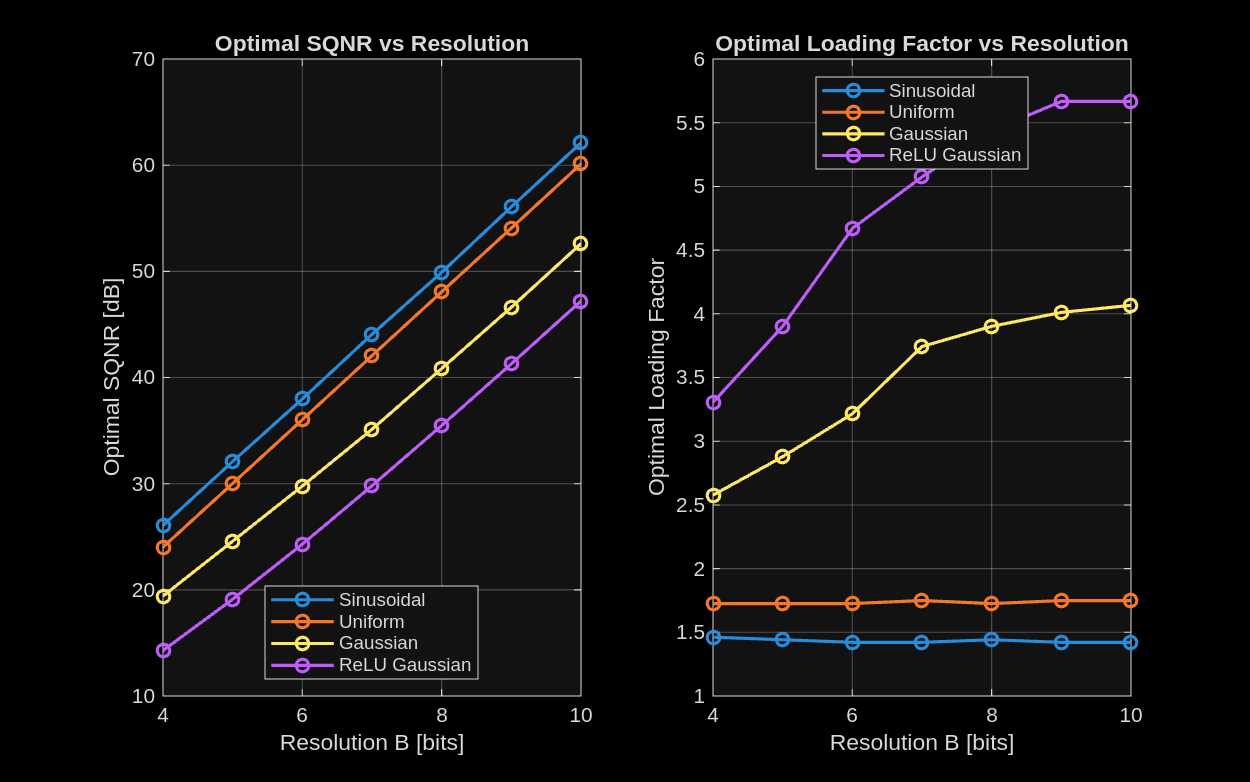
\includegraphics[width=0.95\textwidth]{p4_optimal_sqnr_and_lf.png}
      \caption{Left: optimal SQNR vs resolution. Right: optimal loading factor vs resolution.}
      \label{fig:optimal}
  \end{figure}

  \subsection{Observations}

  \begin{enumerate}
      \item The sinusoidal input achieves the highest SQNR at each resolution because its bounded amplitude allows the quantizer
   to be loaded optimally without clipping.
      \item The Gaussian input requires a larger loading factor (wider FSR) to accommodate its tails, trading quantization
  precision for reduced clipping distortion.
      \item The ReLU Gaussian, being unipolar, is less efficiently matched to the bipolar mid-rise quantizer, resulting in the
  lowest SQNR.
      \item For all signals, SQNR increases by $\approx$6\,dB per bit at the optimal loading factor, confirming the $6.02B$ rule
   of thumb.
      \item The optimal loading factor is signal-dependent and approximately constant across resolutions for each type of signal.
  \end{enumerate}

    \section{SQNR Calculation}

  \subsection{Setup}

  \begin{itemize}
      \item Ideal quantizer, $B = 14$ bits
      \item Input: periodic full-scale half-wave rectified sinusoid with amplitude $A$ and period $T$
      \item Statistical quantizer model applies (sufficiently randomized samples)
  \end{itemize}

  \subsection{Signal Power}

  The half-wave rectified sinusoid is defined as:
  \[
      v_{in}(t) = \begin{cases}
          A\sin\!\left(\dfrac{2\pi t}{T}\right) & 0 \leq t \leq T/2 \\[4pt]
          0 & T/2 < t \leq T
      \end{cases}
  \]

  Its time-averaged power is:
  \begin{align}
      P_{sig} &= \frac{1}{T}\int_0^{T} v_{in}^2(t)\,dt
      = \frac{1}{T}\int_0^{T/2} A^2 \sin^2\!\left(\frac{2\pi t}{T}\right)dt \nonumber \\[6pt]
      &= \frac{A^2}{2T}\int_0^{T/2}\left[1 - \cos\!\left(\frac{4\pi t}{T}\right)\right]dt
      = \frac{A^2}{2T}\left[\frac{T}{2} - 0\right]
  \end{align}
  \[
      \boxed{P_{sig} = \frac{A^2}{4}}
  \]

  \subsection{Quantization Noise Power}

  The signal is unipolar, spanning $[0,\,A]$. Since it is \emph{full-scale}, the quantizer's full-scale range matches the signal
   range:
  \[
      V_{FS} = A, \qquad \Delta = \frac{V_{FS}}{2^B} = \frac{A}{2^{14}}
  \]

  Under the statistical model, the quantization noise power is:
  \[
      P_q = \frac{\Delta^2}{12} = \frac{A^2}{12 \cdot 2^{28}}
  \]

  \subsection{SQNR Calculation}

  \begin{align}
      \text{SQNR} &= \frac{P_{sig}}{P_q}
      = \frac{A^2/4}{A^2/(12 \cdot 2^{28})}
      = \frac{12 \cdot 2^{28}}{4}
      = 3 \cdot 2^{28}
  \end{align}

  Converting to dB:
  \begin{align}
      \text{SQNR}_{\text{dB}} &= 10\log_{10}\!\left(3 \cdot 2^{28}\right) \nonumber \\
      &= 10\log_{10}(3) + 28 \times 10\log_{10}(2) \nonumber \\
      &= 4.77 + 84.29
  \end{align}
  \[
      \boxed{\text{SQNR} \approx 89.1\;\text{dB}}
  \]

  \subsection{Comparison with Standard Full-Scale Sinusoid}

  For a full-scale sinusoid on a bipolar quantizer, $\text{SQNR} = 6.02B + 1.76 = 86.0$\,dB at $B = 14$.

  The half-wave rectified signal achieves 3\,dB \emph{higher} SQNR despite having half the power of a full sinusoid ($A^2/4$
  vs.\ $A^2/2$). This is because the unipolar signal only requires half the quantizer range ($V_{FS} = A$ instead of $2A$),
  reducing $\Delta$ by a factor of 2 and thus $P_q$ by a factor of 4 ($+6$\,dB). The net effect is $-3 + 6 = +3$\,dB relative to
   the bipolar sinusoidal case.

\end{document}